\documentclass[conference]{IEEEtran}
\IEEEoverridecommandlockouts
% The preceding line is only needed to identify funding in the first footnote. If that is unneeded, please comment it out.
\usepackage{cite}
\usepackage{amsmath,amssymb,amsfonts}
\usepackage{algorithmic}
\usepackage{graphicx}
\usepackage{textcomp}

\def\BibTeX{{\rm B\kern-.05em{\sc i\kern-.025em b}\kern-.08em
    T\kern-.1667em\lower.7ex\hbox{E}\kern-.125emX}}

\begin{document}

\title{AResMan\\
Automatic Resource Management\\
{\footnotesize A system tool for improving servers business continuity}
}

\author{\IEEEauthorblockN{Lorenzo Cipriani}
\IEEEauthorblockA{\textit{Principal Engineer - ICT Operation Competence Center}\\
\textit{Huawei Technologies, Ireland Research Lab}\\
Dublin, Ireland\\
https://github.com/lorenzocipriani/}
}

\maketitle

\begin{abstract}
A server is running but performances are not so good or some service is not responding; the system administrator tries to connect to the system in order to check what is happening, but the client used for the remote connection (SSH o RDP) hangs forever (or it’s really slow); then the administrator tries to access directly to the console (physically or virtually) but the system doesn’t react to the login process. After struggling for about 20 minutes, the system administrator decides to reboot the server, sometimes losing any capability to investigate on the root cause of the issue. 
This scenario is pretty common in business-critical environments and the causes are usually related to internal processes that are exhausting all the system resources, due to internal malfunction or external attacks, like denial of service (DOS) ones. 
This solution aims to always grant administrative access to the system, while tracking how processes are managing the system resources; it’s also capable to decide to restart or stop the services that are causing system resource usage excesses. 
\end{abstract}

\begin{IEEEkeywords}
system access; resource management; business continuity
\end{IEEEkeywords}

\section{Introduction}
\subsection{Background}
A server running in a server farm is not (easily) physically accessible to its system administrators. There are tools to remotely access to its console (kvm, ssh, rdp, etc.). 

When a system is under a DOS attack or an application is running and not handling system resources properly, it can be impossible for a system operator to access the system, check what’s going on and do any action that is required to bring the system back to a healthy state.

In some conditions, it’s not possible to access even if the operator was on site, because all the system resources are taken, several processes are stuck and even a simple login to the system is denied due to process timeout.

In this case, the only action the system administrator can do is to proceed with a reboot of the system. Losing any opportunity to investigate the problem while was happening and disrupting the services that the system is supposed to provide.

During my professional experience, I saw this scenario happening several times. No matter if the server was Linux, BSD or Windows, if the system has not been properly configured at deploy time for an accurate resource management - and kept updated while the business requirements changed overtime - the denial of the access to the system administrator is always possible.

When this issue affects the system component that is responsible for monitoring and logging, then it’s impossible to conduct any investigation on the problem because there are no evidences that can be used.

In the usual “2 opposite views” of the IT world the developers expect that system administrators would take care of the system configuration in order to contains their software into the system limits, on the other side the system administrators expect that the software that is required to be installed on a system has an internal check of the resources in order to avoid usage excesses or, at least a configuration and tuning documentation that has been written after the system verification tests (SVTs). Daily practice shows that both statements are false and, especially in those environments where several products are integrated together.

In order to guarantee the access to a system even when a proper configuration is missing and the resources are nearly exhausted, I looked for a solution that could be able to automatically control how much any process in a system is trying to consume from it and that is able to take decisions on their management, including the critical ones like restarting or definitely stopping a service - or even kill the process if a clean stop is not executed in an expected amount of time, but I haven’t found anything like that, so far. 

On the most recent versions of the Linux kernel, the Control Groups (cgroups) \cite{b1} – a feature that limits, accounts for, and isolates the resource usage of a collection of processes - could be used to avoid the described scenario, but (again) it’s not available “out-of-the-box” and it requires an adequate planning and configuration to be used.

\subsection{Aims}
The goal of this project was to develop a service that preserves the business continuity of a system when an unplanned/unmanaged high load is taking most of its resources and it becomes unresponsive.

The application is able to work autonomously as-is, so it’s effective even if the system administrator hasn’t configured it.

The solution relies on 2 main aspects:
\begin{itemize}
\item Grant higher priority at the kernel scheduler to some essential processes like sshd, tty, login and the tool itself
\item Manage directly those processes that are slowing down the system and taking “too much” resources.
\end{itemize}

”Too much” is determined by the algorithm and the tuning capabilities given by the tool configuration.

In this way, if a server is under DOS attack or a process/service is having an odd behavior, a system administrator is always able to open an ssh connection, login to the system, investigate the root cause of the issue and take the proper countermeasures.

There are some alternatives to manage system resources and avoid system denials, but all of them are based on an accurate resource allocation plan and configuration. This solution aims to be ready to work with little or no configuration. 

The advantages of this solution are that a System Administrator will always be able to access to a busy server in order to analyze the problem and choose the right actions to fix the system. On the other side the disadvantages are related to the availability of services that will be slowed down or stopped/restarted if necessary. However, in a clustered environment, these disadvantages could be limited to a reduced capacity instead of a complete service disruption.

The initial configuration of the algorithm cannot satisfy all the customer’s scenarios, thus, for responding to particular needs, the application can be tuned with a configuration file.

\subsection{Technologies}
In order to work with system resources and use directly some kernel features, the application must be compiled in machine code, so C programming language has been chosen for the application development. 
An alternative has also been evaluated during the first couple of weeks of the project: GO. It’s less complex than C in some aspects and it has an easier portability (multiplatform) but is limited to BSD, Linux, Mac OS X and Windows. However, this option has been discarded after the A/B test made in order to compare C and GO.
Finally, because of several issues discovered during the development phase (cross-platform compilation, direct memory allocation and protection, etc.), this choice needed to be reviewed for being able to complete the project within the deadline. Therefore, the solution used for testing, it has been re-written in Python.
No external frameworks have been used for the development this application and the libraries included are:
\begin{itemize}
\item C
  \begin{itemize}
  \item GNU C Standard Library
  \end{itemize}
\item Python
  \begin{itemize}
  \item Standard Python 2.7 packages 
  \end{itemize}
\end{itemize}
Some tools, instead, have been used for the build toolchain and the final test:
\begin{itemize}
\item GNU Autotools (autoconf, automake, etc.) has been used in the first phase of the project in order to facilitate the application build, but it has been abandoned because the porting from Mac OS X (the platform used for development and unit tests) to Linux (the platform used for the final build and run) was raising several errors and trying to fix all of them caused too much delay
\item CMake a tool that manages the build process in an operating system, following a compiler-independent approach. This tool successfully handled the Mac > Linux compile issues as well as the Windows > Linux ones
\item Oracle VirtualBox for hosting a virtual machine with restricted hardware specs (1-2 CPUs, 512-2048 MB ram) where the application is installed
\item Apache Jmeter for simulating a high number of concurrent HTTP requests (5-10,000 threads for 10,000-100,000 loops) against the virtual machine
\end{itemize}

\section{System}

\subsection{Requirements}

\subsubsection{Functional Requirements}
\begin{itemize}
\item The application must run as a service daemon.
\item The application must reserve and lock a memory area in order to have it always available for tracking the system metrics.
\item The application must continuously monitor the system resources with a defined interval of time.
\item The application must change (increase) its own scheduler priority.
\item The application must change (increase) the scheduler priority of the getty, login and ssh processes.
\item The application must change (decrease) the scheduler priority of the processes that are taking too many resources.
\item The application must restart or eventually stop those processes that are taking too many resources from the system.
\end{itemize}
\subsubsection{Data Requirements}
\begin{itemize}
\item The application must read the operating system metrics from the kernel.
\item The application must read the full process list of the system.
\item The application must read the CPU metrics.
\item The application must read the memory metrics.
\item The application must read the disk I/O metrics.
\item The application must read the network I/O metrics.
\end{itemize}
\subsubsection{User Requirements} ~\\
None.
\subsubsection{Environmental Requirements}
\begin{itemize}
\item The application must be started with the operating system.
\item The application must run as root/administrator.
\item The application must have the lowest overhead possible on the system.
\end{itemize}
\subsubsection{Usability Requirements} ~\\
None.

\subsection{Design and Architecture [Figure~\ref{componentDiagramFull}]}

\begin{figure*}[!tbp]
\makebox[\textwidth][c]{\centerline{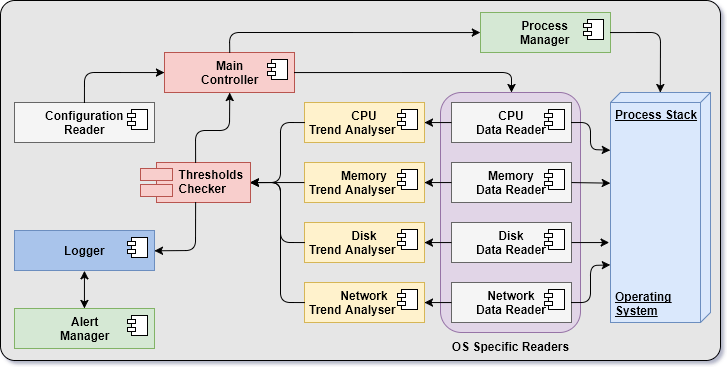
\includegraphics[width=\textwidth]{./img/ComponentDiagram.png}}}
\caption{Component Diagram.\label{componentDiagramFull}}
\end{figure*}

The application starts at system boot and permanently runs with a small CPU \& memory footprint (low overhead).

It runs with reserved “not-pageable” memory and a high CPU priority that is just one-five levels below the kernel ones but much higher than the standard user processes, in order to be reactive even when all the resources of the system are taken.

When application starts, first checks that some necessary processes for accessing the system (getty, login and ssh) in the user space are running with an adequate priority; then the application continuously monitors system resources and is able to automatically take decision in order to keep the system running and guarantee the access to the system to its administrators.

The application uses an algorithm that takes as an input some metrics: CPU, Memory, Swap, Disk I/O, Network I/O, I/O wait state; and is able to use that data for managing processes and interfaces that got stuck and recovering their availability.

\subsection{Implementation}
These values are read when the application starts:
\begin{itemize}
\item CPU: number of CPUs
\item Memory: total physical memory, total swap space
\item Disk: total space for each partition
\end{itemize}
These system metrics are read every X (60) seconds and kept in memory for Y (30) minutes as an input and compared to the previous values:
\begin{itemize}
\item CPU – usage \%
\item Memory – available, free, used of physical and swap spaces
\item Disk – available space for each partition
\item Processes – I/O wait state, cpu and memory usage
\end{itemize}
Triggers for the algorithm to take action:
\begin{itemize}
\item CPU usage over 98\%, memory usage over 95\%, swap space usage over 95\%, process I/O wait state over 5\%
\end{itemize}
When a trigger is activated, the application reduces the priority at the kernel scheduler of the process/es that is/are giving problems. For a set of known processes (by default or by configuration) a restart/stop action is submitted to the process/es.

\subsection{Testing}

\subsubsection{How to test the solution} ~\\
A virtual machine that runs as an HTTP server is installed as a test server. 

A tool that simulates a high number of http requests runs on another system

A tool that uses a lot of system resources is installed on the test server and let it run during the test.

The solution is installed on the test server.

\subsection{Graphical User Interface (GUI)}
The solution is a system service that runs without user interface and is detached by any console, so the only output is the application log.

\subsection{Customer Testing}
No customer testing has been run yet. The solution still needs to be deployed on a production environment after a set of system verification tests and system integration tests.

\subsection{Evaluation}
To evaluate the solution in the test environment, the only 2 checks that can be done are:
\begin{itemize}
\item There are no processes in the systems that are taking more resources that the one defined in the thresholds.
\item The system allows to be accessed also while the load test it’s running at the highest values.
\end{itemize}

Two scenarios are used to measure the effects of the solution: 
\begin{itemize}
\item When the application is stopped and the tools that overload the test server are running, an access to the system is attempted and the time required to successfully login to the system is recorded.
\item Another test cycle will have the application running while the system is artificially overloaded, an access to the system is attempted and the time required to successfully login to the system is recorded and compared to the previous scenario.
\end{itemize}

\section{Conclusions}
The solution seems to respond to most of the requirements, however, given that was not possible to reproduce in the test environment a real system failure due to high resource usage, before considering this project complete and, eventually, usable in production, we need to wait for the SVT and SIT stages to be completed.

The opportunities of this solution are related to the capability of the tool to take decisions automatically for saving essentials system resources. Moreover, the solution has an algorithm that can work as-is without any configuration. However, this could be also a limit of the solution in some scenarios where the tool could “sacrifice” services causing disruptions to the end users. For these particular cases, a fine-grained configuration is required to drive the algorithm to an acceptable behavior.

\section{Further Development or Research}

\subsection{Inclusion in the main Linux distribution repositories}

After a period of use in a real production environment, if this solution still satisfies the expectations, it could be promoted to be included as part of the principal Linux Server distributions. It’s an alternative approach to other resource management solutions (e.g.: cgroups) that require a good implementation design and a proper (manual) configuration during the system deployment. Working “out of the box”, will grant to access to busy systems even if their administrators forgot to configure them properly.

\subsection{Porting to Windows platform}

Changing the OS specific readers components (CPU, Memory, Disk, Network) with the Windows specific ones, the solution can work on that server system too.

\subsection{Machine-Learning engine}

A component of machine learning algorithms can be added to the basic solution in order to improve the analysis capabilities of the trend analyzers and to automatically tune the proper thresholds for each metric into the thresholds checker component.

\begin{figure}[	!htbp]
%\makebox[\textwidth]{\framebox[\textwidth]{\rule{0pt}{2.5cm}}}
\centerline{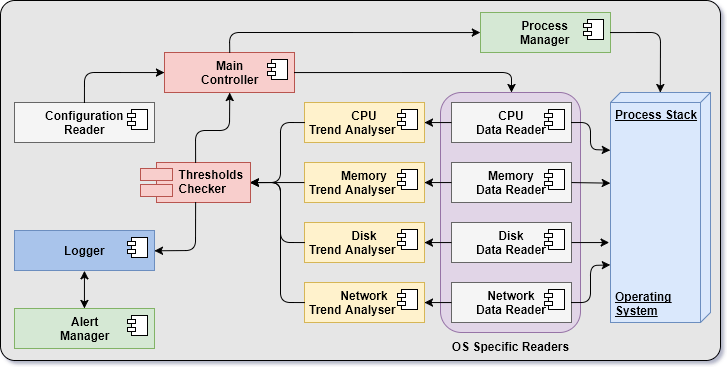
\includegraphics[width=0.5\textwidth]{./img/ComponentDiagram.png}}
\caption{Component Diagram.\label{componentDiagram}}
\end{figure}

\begin{thebibliography}{00}
\bibitem{b1} P. Menage and R. Seth, "cgroups," Wikipedia, [Online]. Available: https://en.wikipedia.org/wiki/Cgroups.
\bibitem{b2} P. Mochel, The sysfs Filesystem, 2005.
\bibitem{b3} D. Watson, "Linux Daemon Writing HOWTO", v1.0, May 2004, [Online].
\bibitem{b4} "The GNU C Library", [Online].
\end{thebibliography}

\end{document}
